\thispagestyle{empty}
\textbf{IMPORTANTE:} Spectrasoft es un software para la utilizaci\'{o}n del espectrofot\'{o}metro MiniScan XE Plus con manejo de bases de datos, por lo tanto es un producto de instalaci\'{o}n y configuraci\'{o}n complejas. Por esta raz\'{o}n se aconseja que la instalaci\'{o}n sea realizada por un t\'{e}cnico o profesional en el \'{a}rea de inform\'{a}tica y de bases de datos.

Este manual se debe leer de principio a fin, siguiendo los pasos al pie de la letra y en el orden que dicta el mismo. No cumplir esto puede causar una instalaci\'{o}n, configuraci\'{o}n y/o ejecuci\'{o}n defectuosa del producto.

Las instalaciones y configuraciones previas a la instalaci\'{o}n del Spectrasoft se deben realizar una sola vez en el sistema. En caso de que sea necesaria la reinstalaci\'{o}n del Spectrasoft, no ser\'{a} necesaria la reinstalaci\'{o}n ni reconfiguraci\'{o}n de los paquetes previos.
\newpage
\section{Requerimientos del sistema}

\subsection{Requerimientos de hardware}

	\begin{itemize}
		\item Procesador de 1 gigahertz (GHz) o superior.
		
		\item 1 gigabyte (GB) de memoria RAM o m\'{a}s.
		
		\item Resoluci\'{o}n de pantalla de 1024x768 o superior.
	\end{itemize}
	
\subsection{Requerimientos de arquitectura}

	\begin{itemize}
		\item Arquitectura de 32 bits o de 64 bits.
	\end{itemize}

\subsection{Requerimientos del sistema operativo}

	\begin{itemize}
		\item Sistema operativo Microsoft Windows 7 Service Pack 1 o superior.
	\end{itemize}
	
\subsection{Requerimientos de software}

	\begin{itemize}
		\item Microsoft .NET framework 4 o superior.
		
		\item Microsoft Internet Explorer 10 o superior.
	\end{itemize}

\newpage

\section{Acciones previas}

	\subsection{Controlador para el adaptador serial-USB}
	
	Conecte el MiniScan XE Plus utilizando el cable adaptador serial-USB, luego instale el controlador para el adaptador dejando todas las opciones de instalaci\'{o}n por defecto.

	\subsection{Paquete MSXP-CFLX Utility}
	
	Instale el paquete MSXP-CFLX Utility, ejecut\'{a}ndolo como administrador y dejando todas las opciones de instalaci\'{o}n por defecto.
	
	\subsection{Carpeta MSXEBridge}
	
	Copie la carpeta <<MSXEBridge>> en el disco local C, en la ruta <<C:\textbackslash>>.
	
\section{Versiones de los paquetes a instalar}

\begin{itemize}
	\item Visual Studio 2013 community/professional/ultimate.
	
	\item PostgreSQL 9.4.4-3.
\end{itemize}

\newpage

\section{Instalaci\'{o}n de Visual Studio}
	
Ejecute la instalaci\'{o}n de Visual Studio como administrador. Seleccione la opci\'{o}n <<Acepto los t\'{e}rminos de licencia y la declaraci\'{o}n de privacidad.>> y haga click en el bot\'{o}n <<Siguiente>> (v\'{e}ase la figura \ref{fig:vs-instalacion1}).

\begin{figure}[H]
  \centering
  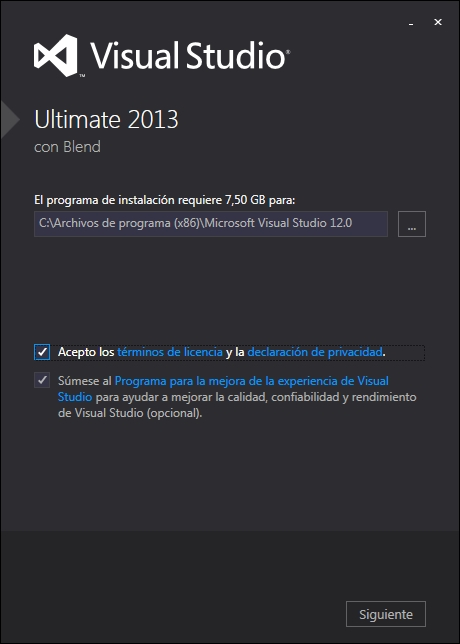
\includegraphics[width=.8\linewidth]{./img/vs-instalacion1.jpg}
\caption[Inicio de instalaci\'{o}n de Visual Studio]{Inicio de instalaci\'{o}n de Visual Studio\label{fig:vs-instalacion1}}
\end{figure}
\newpage
Deje todas las opciones por defecto de <<Caracter\'{i}sticas opcionales para instalar:>> y haga click en el bot\'{o}n <<INSTALAR>> (v\'{e}ase la figura \ref{fig:vs-instalacion2}).	

\begin{figure}[H]
  \centering
  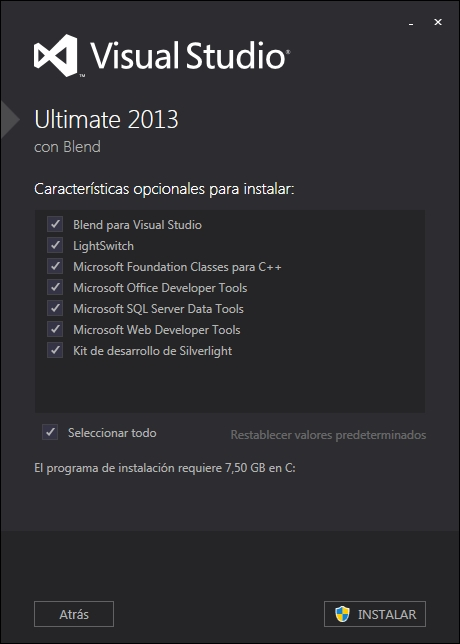
\includegraphics[width=.8\linewidth]{./img/vs-instalacion2.jpg}
\caption[Caracter\'{i}sticas opcionales de Visual Studio]{Caracter\'{i}sticas opcionales de Visual Studio\label{fig:vs-instalacion2}}
\end{figure}
\newpage
Espere a que el proceso de instalaci\'{o}n finalice (v\'{e}ase la figura \ref{fig:vs-instalacion3}).	

\begin{figure}[H]
  \centering
  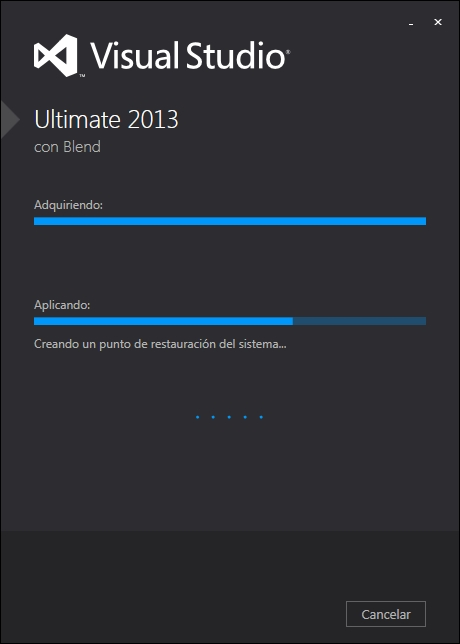
\includegraphics[width=.8\linewidth]{./img/vs-instalacion3.jpg}
\caption[Progreso de la instalaci\'{o}n de Visual Studio]{Progreso de la instalaci\'{o}n de Visual Studio\label{fig:vs-instalacion3}}
\end{figure}
\newpage
Despu\'{e}s de finalizar la instalaci\'{o}n, no inicie Visual Studio, haga click en el bot\'{o}n con forma de equis (x) en la esquina superior para cerrar la ventana (v\'{e}ase la figura \ref{fig:vs-instalacion4}).	

\begin{figure}[H]
  \centering
  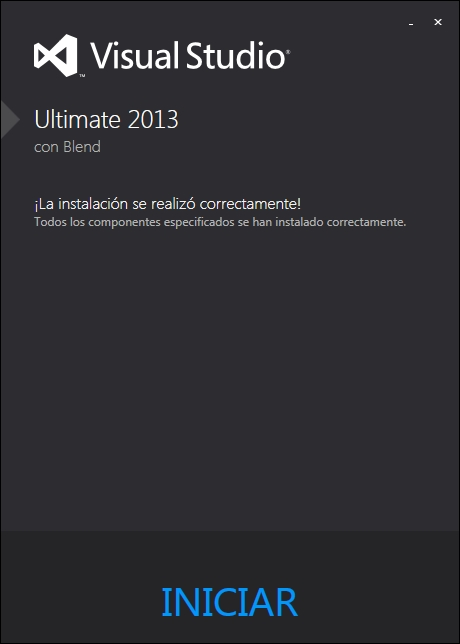
\includegraphics[width=.8\linewidth]{./img/vs-instalacion4.jpg}
\caption[Cerrar ventana de instalaci\'{o}n de Visual Studio]{Cerrar ventana de instalaci\'{o}n de Visual Studio\label{fig:vs-instalacion4}}
\end{figure}

\newpage

\section{Instalaci\'{o}n de PostgreSQL}
	
Ejecute la instalaci\'{o}n de PostgreSQL como administrador. Haga click en el bot\'{o}n <<Siguiente>> (v\'{e}ase la figura \ref{fig:postgres1}).

\begin{figure}[H]
  \centering
  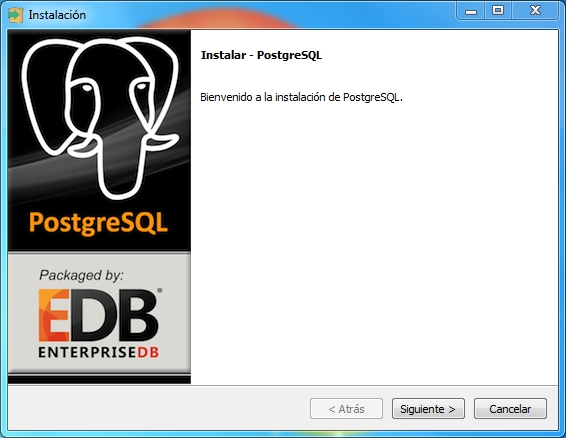
\includegraphics[width=.6\linewidth]{./img/postgres1.jpg}
\caption[Inicio de instalaci\'{o}n de PostgreSQL]{Inicio de instalaci\'{o}n de PostgreSQL\label{fig:postgres1}}
\end{figure}

Deje la ubicaci\'{o}n del directorio de instalaci\'{o}n por defecto y haga click en el bot\'{o}n <<Siguiente>> (v\'{e}ase la figura \ref{fig:postgres2}).

\begin{figure}[H]
  \centering
  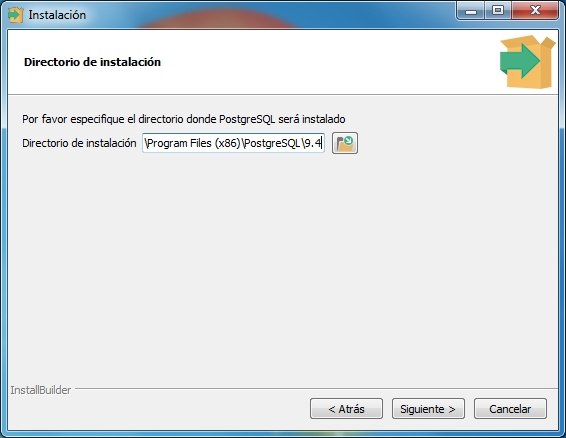
\includegraphics[width=.6\linewidth]{./img/postgres2.jpg}
\caption[Directorio de instalaci\'{o}n de PostgreSQL]{Directorio de instalaci\'{o}n de PostgreSQL\label{fig:postgres2}}
\end{figure}

\newpage

Deje la ubicaci\'{o}n del directorio de datos por defecto y haga click en el bot\'{o}n <<Siguiente>> (v\'{e}ase la figura \ref{fig:postgres3}).

\begin{figure}[H]
  \centering
  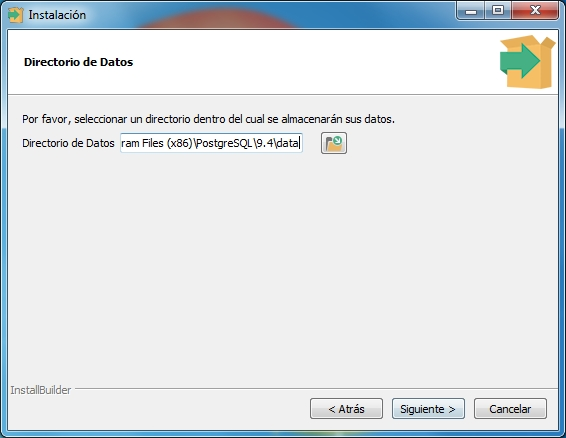
\includegraphics[width=.6\linewidth]{./img/postgres3.jpg}
\caption[Inicio de datos de PostgreSQL]{Inicio de datos de PostgreSQL\label{fig:postgres3}}
\end{figure}

Introduzca una contrase\~{n}a de su preferencia, gu\'{a}rdela en un lugar seguro y haga click en el bot\'{o}n <<Siguiente>> (v\'{e}ase la figura \ref{fig:postgres4}).

\begin{figure}[H]
  \centering
  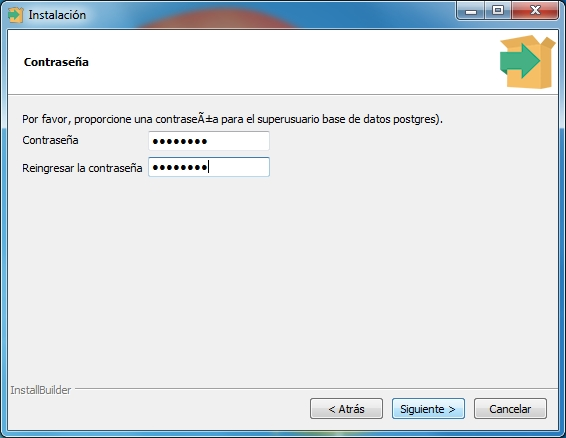
\includegraphics[width=.6\linewidth]{./img/postgres4.jpg}
\caption[Contrase\~{n}a para el superusuario de PostgreSQL]{Contrase\~{n}a para el superusuario de PostgreSQL\label{fig:postgres4}}
\end{figure}

\newpage

Deje el n\'{u}mero del puerto por defecto y haga click en el bot\'{o}n <<Siguiente>> (v\'{e}ase la figura \ref{fig:postgres5}).

\begin{figure}[H]
  \centering
  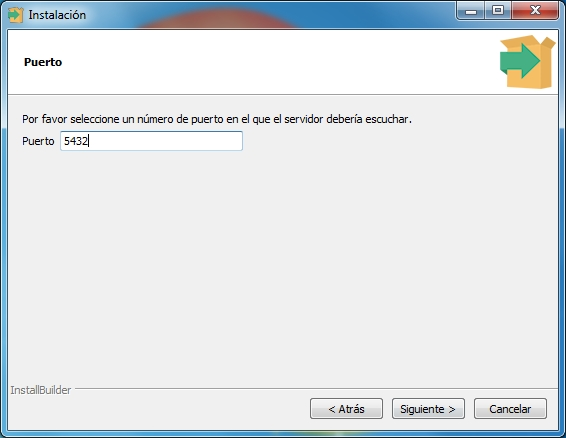
\includegraphics[width=.6\linewidth]{./img/postgres5.jpg}
\caption[N\'{u}mero de puerto para PostgreSQL]{N\'{u}mero de puerto para PostgreSQL\label{fig:postgres5}}
\end{figure}

Deje la configuraci\'{o}n regional por defecto y haga click en el bot\'{o}n <<Siguiente>> (v\'{e}ase la figura \ref{fig:postgres6}).

\begin{figure}[H]
  \centering
  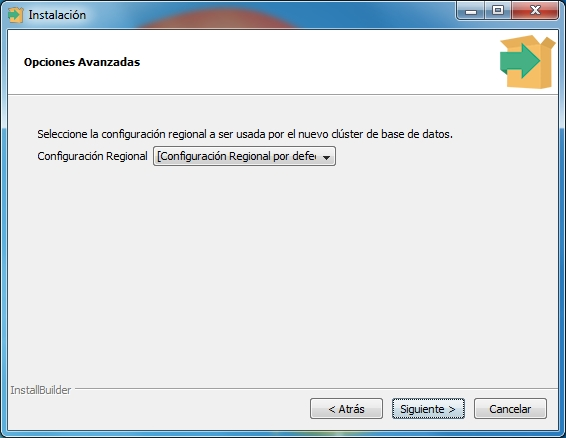
\includegraphics[width=.6\linewidth]{./img/postgres6.jpg}
\caption[Configuraci\'{o}n regional para PostgreSQL]{Configuraci\'{o}n regional para PostgreSQL\label{fig:postgres6}}
\end{figure}

\newpage

Haga click en el bot\'{o}n <<Siguiente>> para empezar el proceso de instalaci\'{o}n y espere a que finalice (v\'{e}ase las figuras \ref{fig:postgres7} y \ref{fig:postgres8}).

\begin{figure}[H]
  \centering
  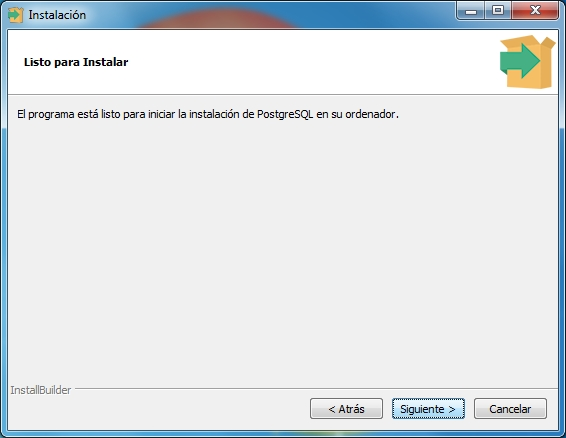
\includegraphics[width=.7\linewidth]{./img/postgres7.jpg}
\caption[Inicio de la instalaci\'{o}n de PostgreSQL]{Inicio de la instalaci\'{o}n de PostgreSQL\label{fig:postgres7}}
\end{figure}

\begin{figure}[H]
  \centering
  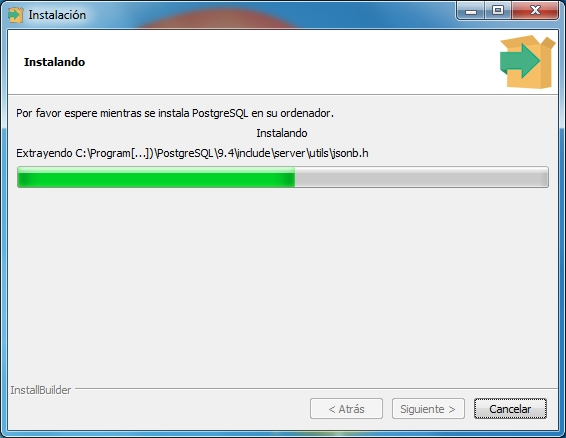
\includegraphics[width=.7\linewidth]{./img/postgres8.jpg}
\caption[Proceso de instalaci\'{o}n de PostgreSQL]{Proceso de instalaci\'{o}n de PostgreSQL\label{fig:postgres8}}
\end{figure}

\newpage

Despu\'{e}s de finalizar la instalaci\'{o}n, aseg\'{u}rese de que la opci\'{o}n <<Lanzar Stack Builder al finalizar>> no este seleccionada, y por \'{u}ltimo haga click en el bot\'{o}n <<Terminar>> (v\'{e}ase la figura \ref{fig:vs-instalacion9}).	

\begin{figure}[H]
  \centering
  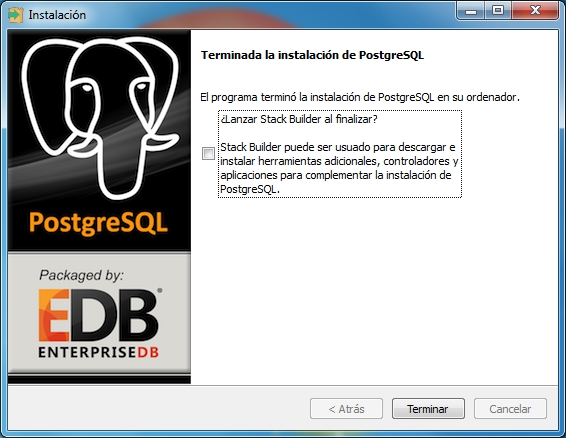
\includegraphics[width=.8\linewidth]{./img/postgres9.jpg}
\caption[Finalizaci\'{o}n de la instalaci\'{o}n de PostgreSQL]{Finalizaci\'{o}n de la instalaci\'{o}n de PostgreSQL\label{fig:vs-instalacion9}}
\end{figure}

\newpage

\section{Configuraci\'{o}n de Visual Studio}
	
	Ejecute el software Visual Studio como administrador. En caso de que al iniciar se le pregunte si desea iniciar sesi\'{o}n, elija la opci\'{o}n <<De momento no, quiz\'{a}s m\'{a}s tarde>> (v\'{e}ase la figura \ref{fig:vs-inicio}).	

\begin{figure}[H]
  \centering
  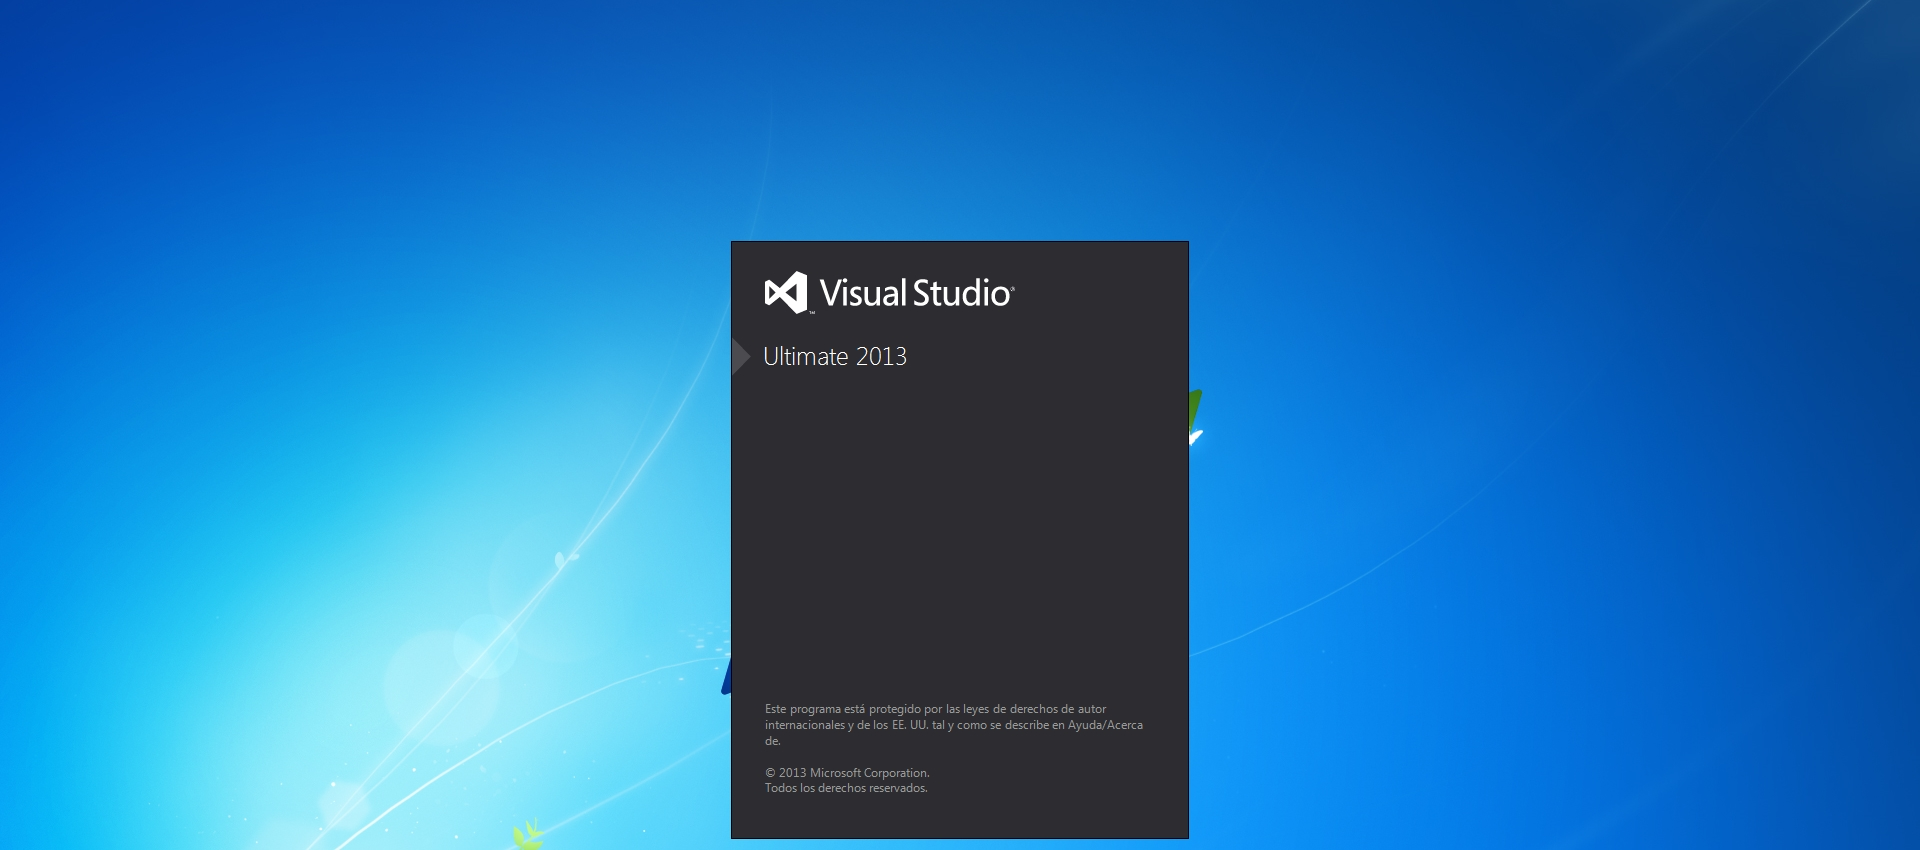
\includegraphics[width=.8\linewidth]{./img/vs-inicio.jpg}
\caption[Vista de inicio de Visual Studio]{Vista de inicio de Visual Studio\label{fig:vs-inicio}}
\end{figure}

En el men\'{u} <<ARCHIVO>> entre al submen\'{u} <<Abrir>> y haga click en la opci\'{o}n <<Proyecto o soluci\'{o}n...>> (v\'{e}ase la figura \ref{fig:vs-abrir}).	

\begin{figure}[H]
  \centering
  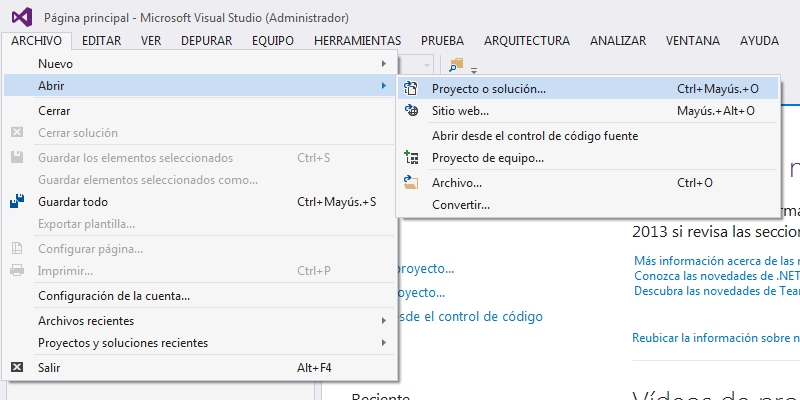
\includegraphics[width=.8\linewidth]{./img/vs-proyecto-abrir.jpg}
\caption[Abrir proyecto]{Abrir proyecto\label{fig:vs-abrir}}
\end{figure}

\newpage

En la carpeta <<MSXEBridge>> ubicada en el disco <<C:\textbackslash>>, seleccione el archivo <<MSXEBridge>> y haga click en el bot\'{o}n <<Abrir>> (v\'{e}ase la figura \ref{fig:vs-abrir-buscar}).

\begin{figure}[H]
  \centering
  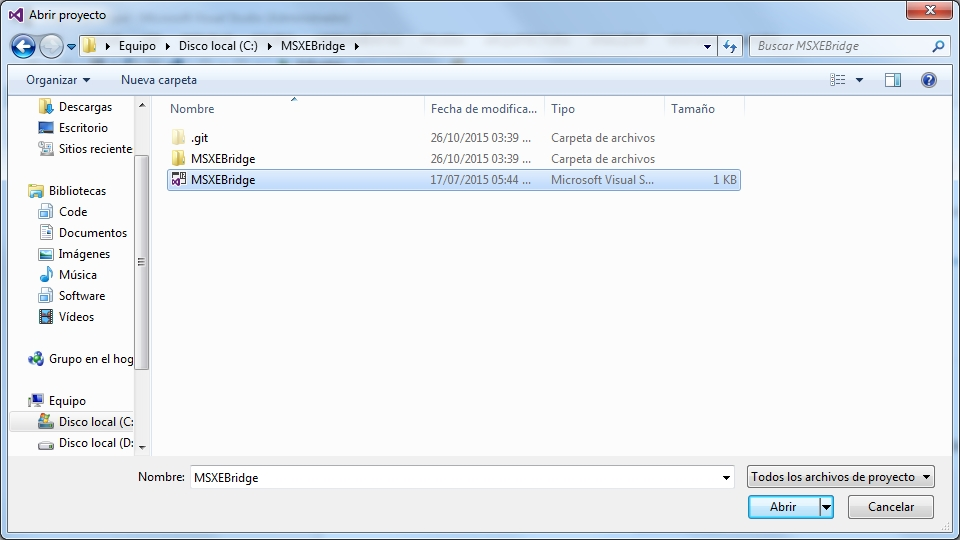
\includegraphics[width=.8\linewidth]{./img/vs-abrir-buscar.jpg}
\caption[Buscar el archivo MSXEBridge]{Buscar el archivo MSXEBridge\label{fig:vs-abrir-buscar}}
\end{figure}

En la parte derecha de Visual Studio, haga click con el bot\'{o}n derecho en <<MSXEBridge>> y seleccione la opci\'{o}n <<Propiedades>> (v\'{e}ase la figura \ref{fig:vs-propiedades}).

\begin{figure}[H]
  \centering
  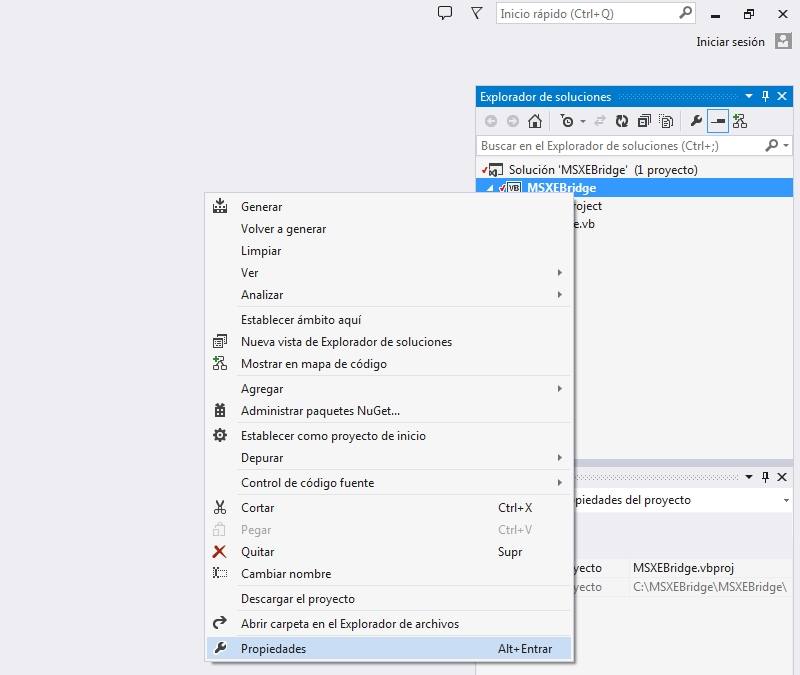
\includegraphics[width=.7\linewidth]{./img/vs-propiedades.jpg}
\caption[Propiedades de MSXEBridge]{Propiedades de MSXEBridge\label{fig:vs-propiedades}}
\end{figure}

\newpage

Haga click al bot\'{o}n <<Informaci\'{o}n de ensamblado...>>, aseg\'{u}rese de que la opci\'{o}n <<Crear ensamblado visible a trav\'{e}s de COM>> est\'{e} seleccionada, y haga click en el bot\'{o}n <<Aceptar>> (v\'{e}ase la figura \ref{fig:vs-ensamblado}).

\begin{figure}[H]
  \centering
  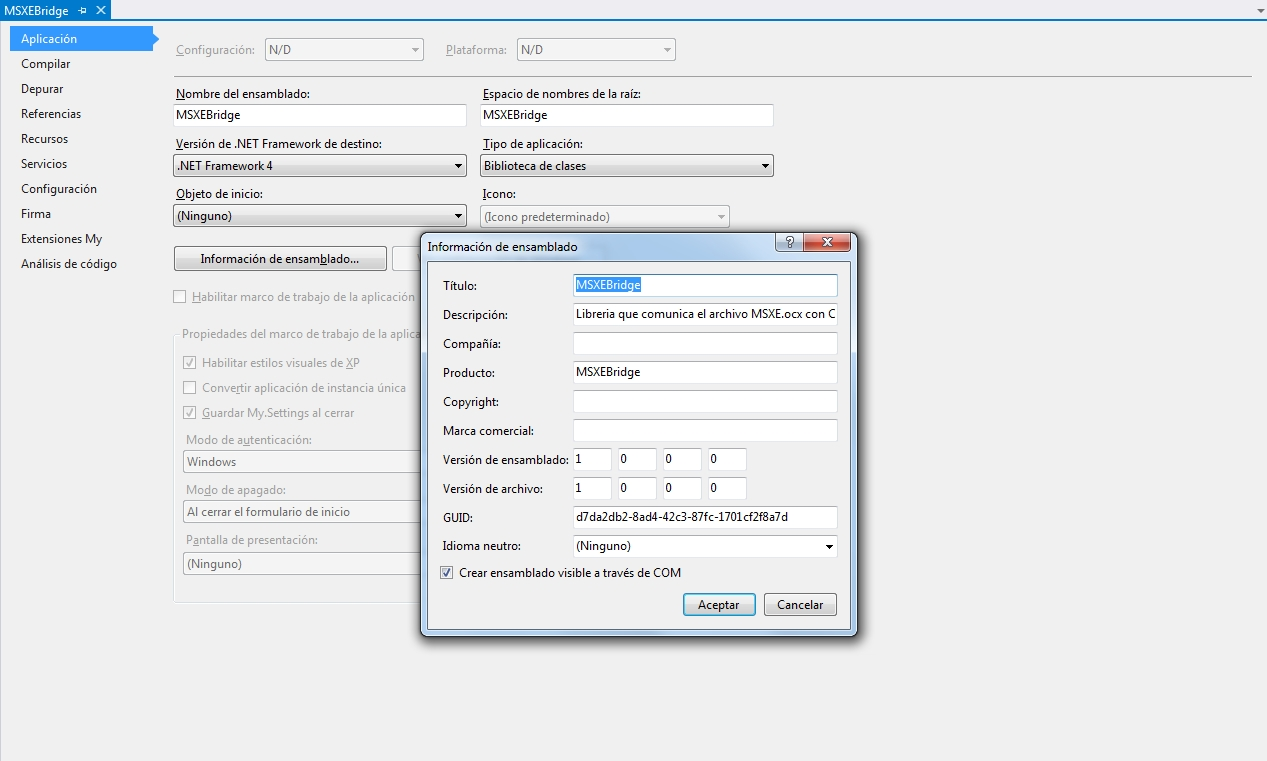
\includegraphics[width=.75\linewidth]{./img/vs-ensamblado.jpg}
\caption[Ensamblado de MSXEBridge]{Ensamblado de MSXEBridge\label{fig:vs-ensamblado}}
\end{figure}

Haga click en la pesta\~{n}a <<Compilar>> y aseg\'{u}rese de que la opci\'{o}n <<Registrar para interoperabilidad COM>> est\'{e} seleccionada (v\'{e}ase la figura \ref{fig:vs-compilar}).

\begin{figure}[H]
  \centering
  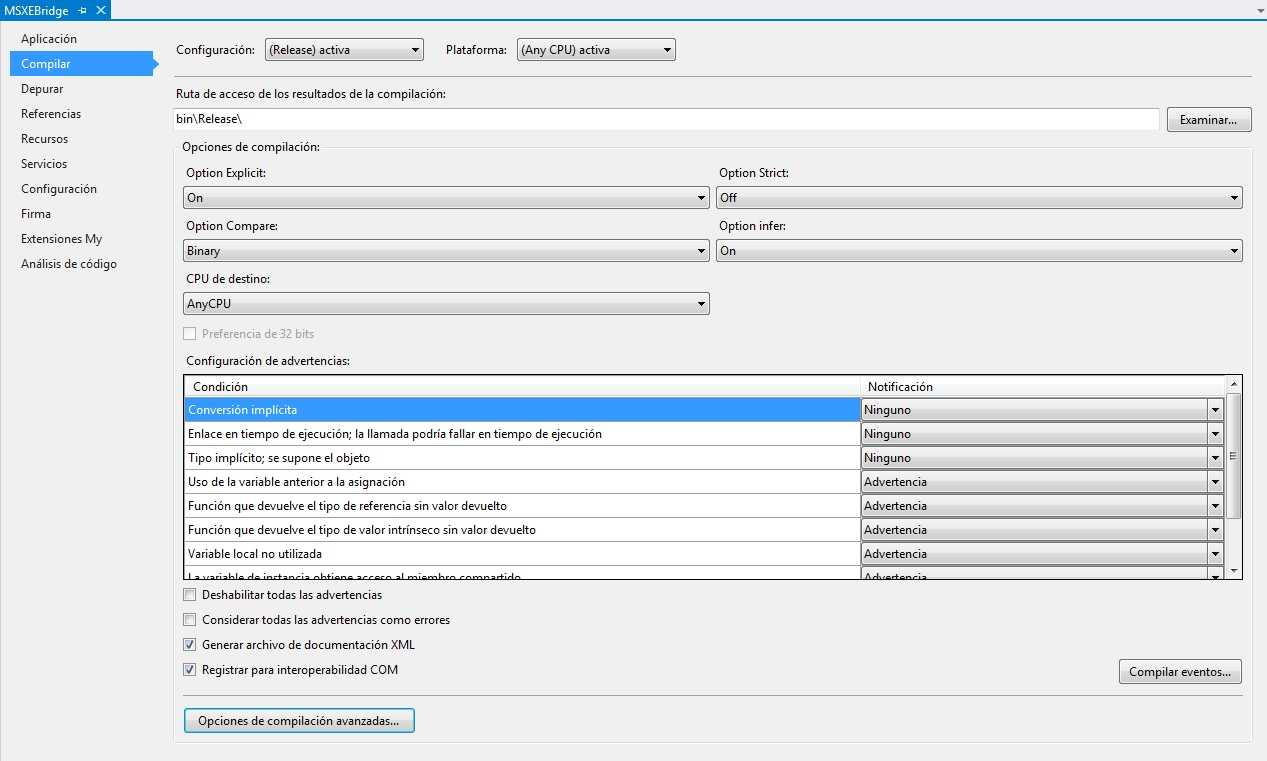
\includegraphics[width=.75\linewidth]{./img/vs-compilar.jpg}
\caption[Interoperabilidad de MSXEBridge]{Interoperabilidad de MSXEBridge\label{fig:vs-compilar}}
\end{figure}

\newpage

En el men\'{u} <<COMPILAR>>, haga click en la opci\'{o}n <<Compilar soluci\'{o}n>> est\'{e} seleccionada (v\'{e}ase la figura \ref{fig:vs-compilar-solucion}).

\begin{figure}[H]
  \centering
  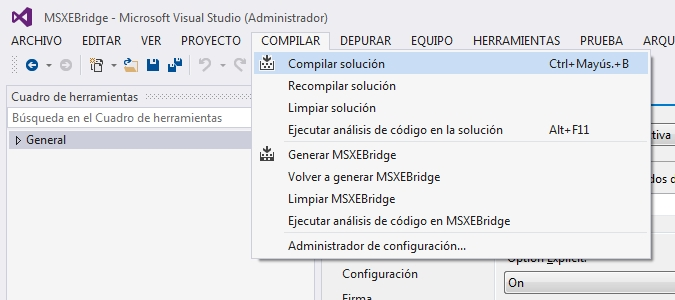
\includegraphics[width=1\linewidth]{./img/vs-compilar-solucion.jpg}
\caption[Compilar MSXEBridge]{Compilar MSXEBridge\label{fig:vs-compilar-solucion}}
\end{figure}

En la parte inferior de Visual Studio podr\'{a} ver que la compilaci\'{o}n finaliz\'{o} correctamente (v\'{e}ase la figura \ref{fig:vs-resultados}). Por \'{u}ltimo, cierre el software Visual Studio.

\begin{figure}[H]
  \centering
  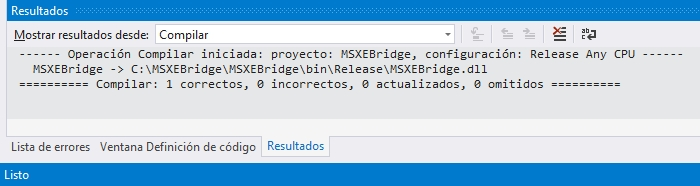
\includegraphics[width=1\linewidth]{./img/vs-resultados.jpg}
\caption[Resultados de la compilaci\'{o}n]{Resultados de la compilaci\'{o}n\label{fig:vs-resultados}}
\end{figure}

Es importante destacar que los pasos seguidos previamente s\'{o}lo se deben realizar una vez, y no es necesario que ejecute Visual Studio posteriormente para ejecutar el Spectrasoft.

\newpage

\section{Configuraci\'{o}n de PostgreSQL}
	
Ejecute el software pgAdmin como administrador (v\'{e}ase la figura \ref{fig:pgadmin-inicio}).
	
\begin{figure}[H]
  \centering
  
\includegraphics[width=1\linewidth]{./img/pgadmin-inicio.jpg}
\caption[Vista de inicio de pgAdmin]{Vista de inicio de pgAdmin\label{fig:pgadmin-inicio}}
\end{figure}

Para accesar al servidor, haga doble click en la opci\'{o}n <<PostgreSQL (localhost:5432)>>, e introduzca la contrase\~{n}a que estableci\'{o} durante el proceso de instalaci\'{o}n (v\'{e}ase la figura \ref{fig:pgadmin-acceso}).

\begin{figure}[H]
  \centering
  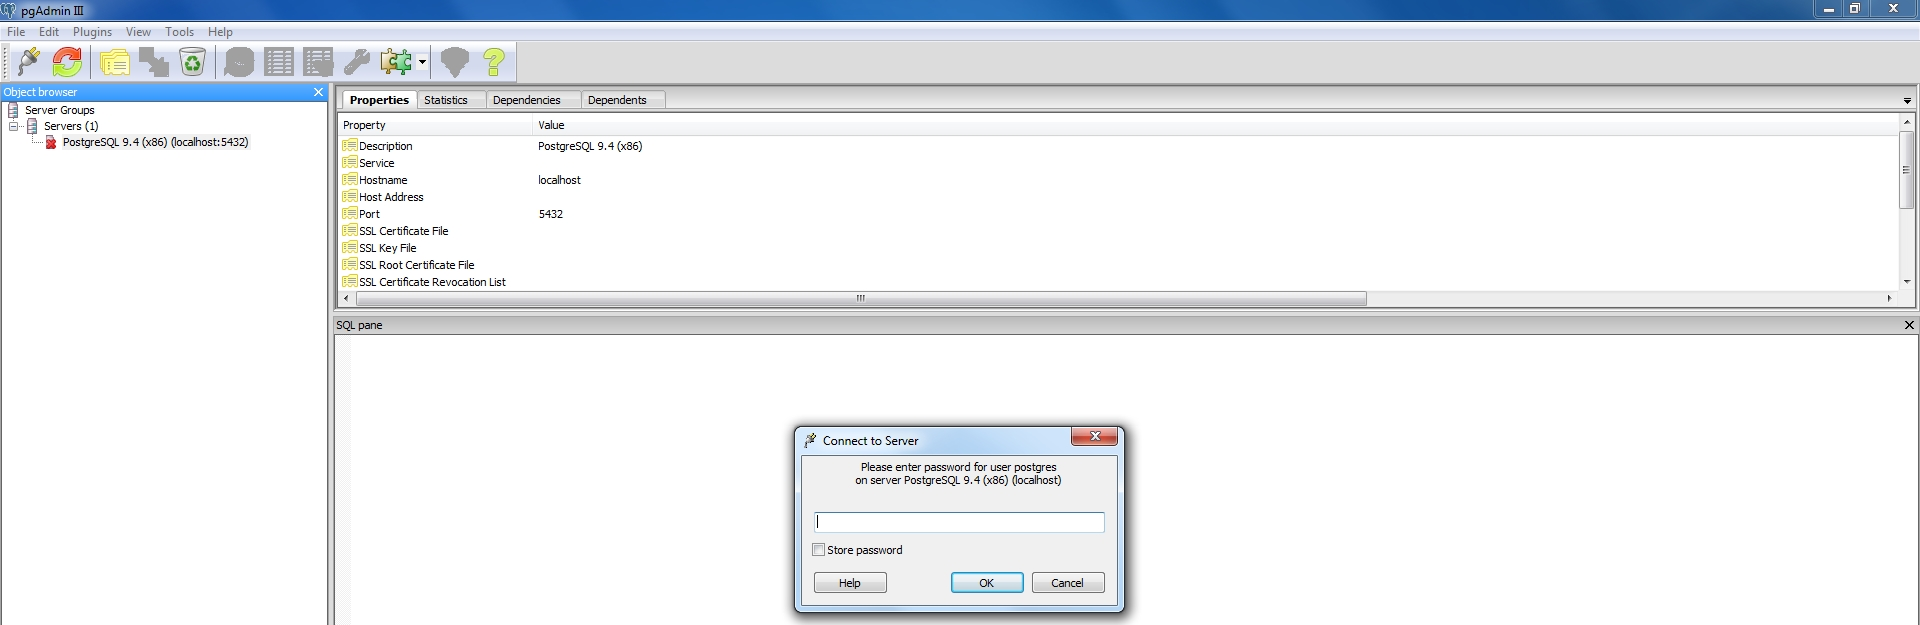
\includegraphics[width=1\linewidth]{./img/pgadmin-acceso.jpg}
\caption[Acceso al servidor]{Acceso al servidor\label{fig:pgadmin-acceso}}
\end{figure}

\newpage

Haga click derecho en el men\'{u} <<Login Roles>> y seleccione la opci\'{o}n <<New Login Role...>> (v\'{e}ase la figura \ref{fig:pgadmin-rol}).

\begin{figure}[H]
  \centering
  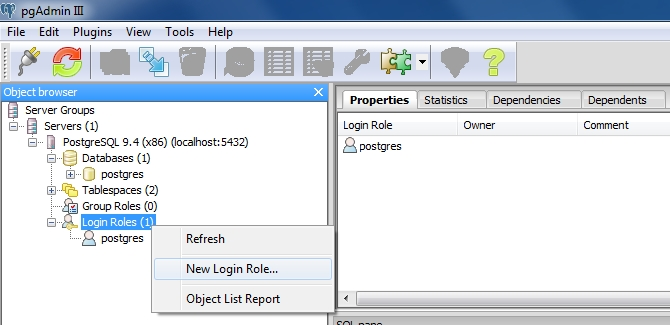
\includegraphics[width=1\linewidth]{./img/pgadmin-rol.jpg}
\caption[Crear nuevo rol]{Crear nuevo rol\label{fig:pgadmin-rol}}
\end{figure}

Introduzca <<CIMBUC>> en <<Role name>> (v\'{e}ase la figura \ref{fig:pgadmin-rol-nombre}).

\begin{figure}[H]
  \centering
  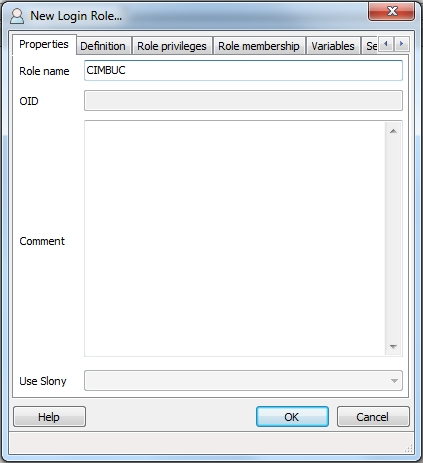
\includegraphics[width=.5\linewidth]{./img/pgadmin-rol-nombre.jpg}
\caption[Nombre del rol]{Nombre del rol\label{fig:pgadmin-rol-nombre}}
\end{figure}

Haga click en la pesta\~{n}a <<Definition>> e introduzca <<CIMBUC>> como la contrase\~{n}a del rol (v\'{e}ase la figura \ref{fig:pgadmin-rol-clave}).

\begin{figure}[H]
  \centering
  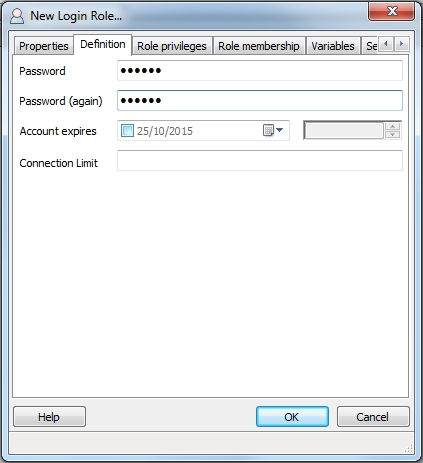
\includegraphics[width=.45\linewidth]{./img/pgadmin-rol-clave.jpg}
\caption[Contrase\~{n}a del rol]{Contrase\~{n}a del rol\label{fig:pgadmin-rol-clave}}
\end{figure}

Haga click en la pesta\~{n}a <<Role privileges>>, seleccione todas las opciones de privilegios disponibles para el rol y haga click en el bot\'{o}n <<OK>> (v\'{e}ase la figura \ref{fig:pgadmin-rol-privilegios}).

\begin{figure}[H]
  \centering
  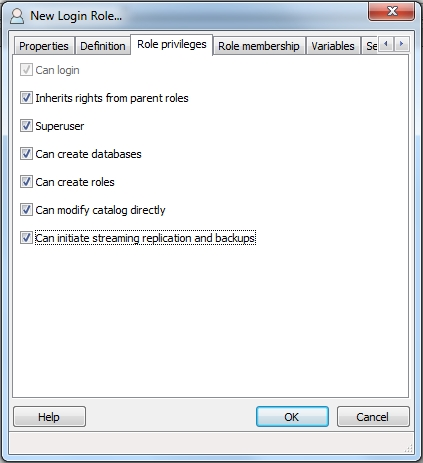
\includegraphics[width=.45\linewidth]{./img/pgadmin-rol-privilegios.jpg}
\caption[Privilegios del rol]{Privilegios del rol\label{fig:pgadmin-rol-privilegios}}
\end{figure}

\newpage

Haga click derecho en el men\'{u} <<Databases>> y seleccione la opci\'{o}n <<New Database...>> (v\'{e}ase la figura \ref{fig:pgadmin-bd}).

\begin{figure}[H]
  \centering
  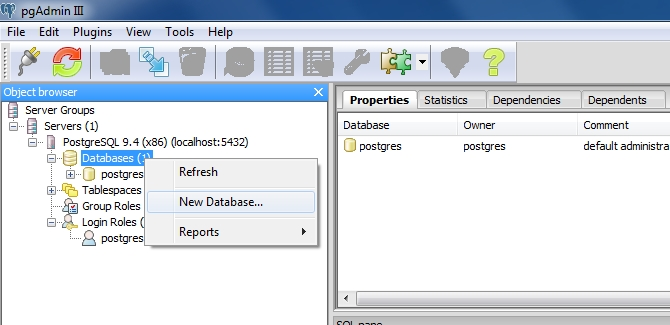
\includegraphics[width=1\linewidth]{./img/pgadmin-bd.jpg}
\caption[Crear nueva base de datos]{Crear nueva base de datos\label{fig:pgadmin-bd}}
\end{figure}

Introduzca <<CIMBUC>> en <<Name>> y haga click en el bot\'{o}n <<OK>> (v\'{e}ase la figura \ref{fig:pgadmin-bd-nombre}).

\begin{figure}[H]
  \centering
  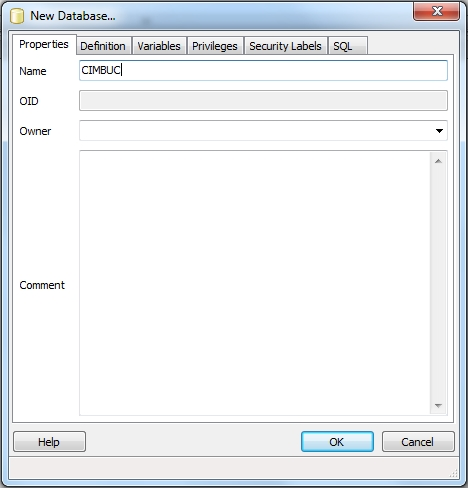
\includegraphics[width=.5\linewidth]{./img/pgadmin-bd-nombre.jpg}
\caption[Nombre de la base de datos]{Nombre de la base de datos\label{fig:pgadmin-bd-nombre}}
\end{figure}

\newpage

Haga click derecho en la base de datos <<CIMBUC>> y seleccione la opci\'{o}n <<Restore...>> (v\'{e}ase la figura \ref{fig:pgadmin-restaurar}).

\begin{figure}[H]
  \centering
  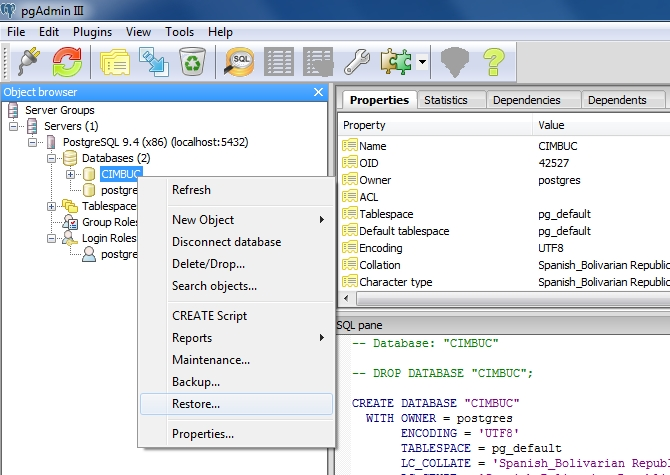
\includegraphics[width=1\linewidth]{./img/pgadmin-restaurar.jpg}
\caption[Opci\'{o}n de restauraci\'{o}n de la base de datos]{Opci\'{o}n de restauraci\'{o}n de la base de datos\label{fig:pgadmin-restaurar}}
\end{figure}

\newpage

Haga click en el bot\'{o}n <<...>> para buscar el archivo de respaldo de la base de datos (v\'{e}ase la figura \ref{fig:pgadmin-restaurar-ventana}).

\begin{figure}[H]
  \centering
  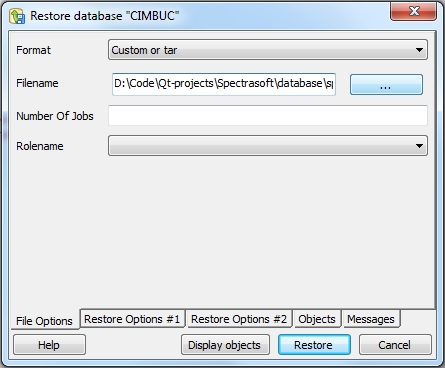
\includegraphics[width=.6\linewidth]{./img/pgadmin-restaurar-ventana.jpg}
\caption[Ventana de restauraci\'{o}n de la base de datos]{Ventana de restauraci\'{o}n de la base de datos\label{fig:pgadmin-restaurar-ventana}}
\end{figure}

Busque y seleccione el archivo <<spectradb.backup>>, y haga click en el bot\'{o}n <<Abrir>> (v\'{e}ase la figura \ref{fig:pgadmin-restaurar-buscar}).

\begin{figure}[H]
  \centering
  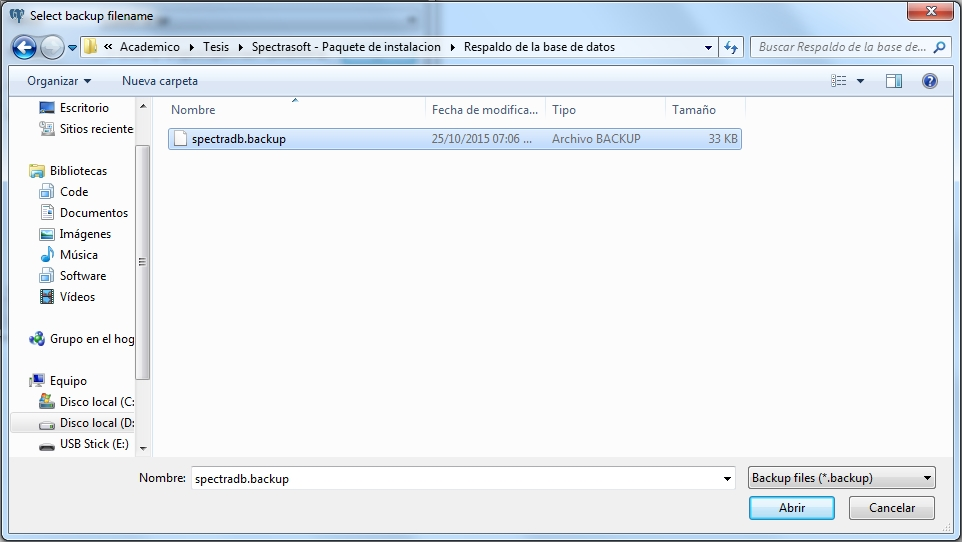
\includegraphics[width=1\linewidth]{./img/pgadmin-restaurar-buscar.jpg}
\caption[Buscar el archivo de respaldo]{Buscar el archivo de respaldo\label{fig:pgadmin-restaurar-buscar}}
\end{figure}

\newpage

De vuelta a la ventana de restauraci\'{o}n, haga click en la lista desplegable de <<Rolename>> y seleccione la opci\'{o}n <<CIMBUC>> (v\'{e}ase la figura \ref{fig:pgadmin-restaurar-rol}).

\begin{figure}[H]
  \centering
  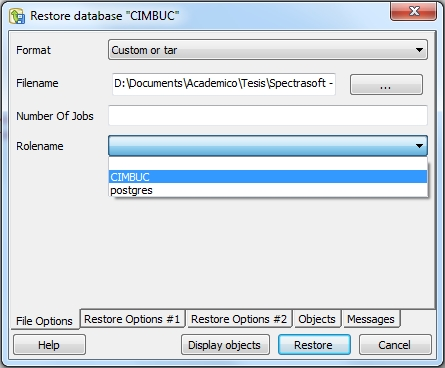
\includegraphics[width=.6\linewidth]{./img/pgadmin-restaurar-rol.jpg}
\caption[Rol de restauraci\'{o}n de la base de datos]{Rol de restauraci\'{o}n de la base de datos\label{fig:pgadmin-restaurar-rol}}
\end{figure}

Haga click en la pesta\~{n}a <<Restore Options \#1>> y en el grupo <<Sections>> seleccione las opciones <<Pre-data>>, <<Data>> y <<Post-data>>, luego haga click en el bot\'{o}n <<Restore>> (v\'{e}ase la figura \ref{fig:pgadmin-restaurar-opciones}).

\begin{figure}[H]
  \centering
  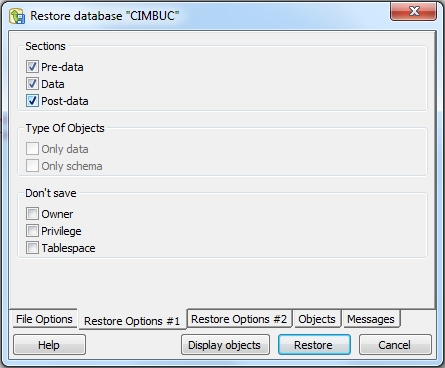
\includegraphics[width=.6\linewidth]{./img/pgadmin-restaurar-opciones.jpg}
\caption[Opciones de restauraci\'{o}n de la base de datos]{Opciones de restauraci\'{o}n de la base de datos\label{fig:pgadmin-restaurar-opciones}}
\end{figure}

\newpage

En la misma ventana haga click en bot\'{o}n <<Done>>, y por \'{u}ltimo cierre el software pgAdmin (v\'{e}ase la figura \ref{fig:pgadmin-restaurar-listo}).

\begin{figure}[H]
  \centering
  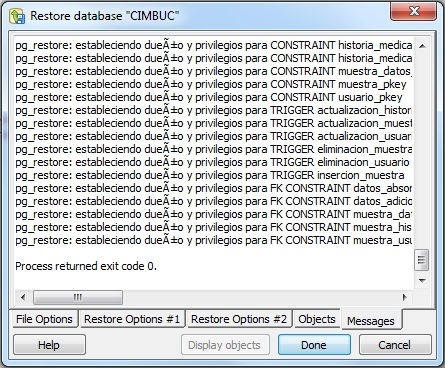
\includegraphics[width=.6\linewidth]{./img/pgadmin-restaurar-listo.jpg}
\caption[Restauraci\'{o}n de la base de datos completa]{Restauraci\'{o}n de la base de datos completa\label{fig:pgadmin-restaurar-listo}}
\end{figure}

Es importante destacar que los pasos seguidos previamente s\'{o}lo se deben realizar una vez, y no es necesario que ejecute pgAdmin posteriormente para ejecutar el Spectrasoft.

La base de datos posee un usuario administrador por defecto para iniciar sesi\'{o}n y trabajar con el Spectrasoft, sus datos de ingreso son los siguientes: 

\begin{itemize}
	\item \textbf{C\'{e}dula de identidad:} V00000000
	
	\item \textbf{Contrase\~{n}a:} 12345Admin
\end{itemize}

Luego de iniciar sesi\'{o}n en el Spectrasoft con este usuario, puede crear otro usuario administrador de su preferencia y eliminar este.

\section{Instalaci\'{o}n del Spectrasoft}

Ejecute el instalador <<setup-spectrasoft>> y haga click en el bot\'{o}n <<Next>>, dejando todas las opciones por defecto hasta llegar al acuerdo de licencia (v\'{e}ase la figura \ref{fig:spectrasoft-setup}).

\begin{figure}[H]
  \centering
  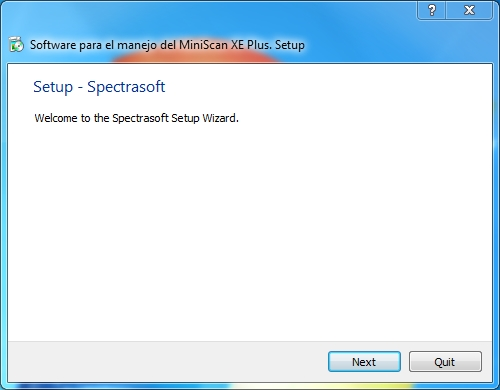
\includegraphics[width=.5\linewidth]{./img/spectrasoft-setup.jpg}
\caption[Instalador del Spectrasoft]{Instalador del Spectrasoft\label{fig:spectrasoft-setup}}
\end{figure}

En la ventana <<License Agreement>>, seleccione la opci\'{o}n <<I accept the license>> y haga click en el bot\'{o}n <<Next>> (v\'{e}ase la figura \ref{fig:spectrasoft-licencia}). Deje las siguientes opciones por defecto hasta llegar la opci\'{o}n de instalar.

\begin{figure}[H]
  \centering
  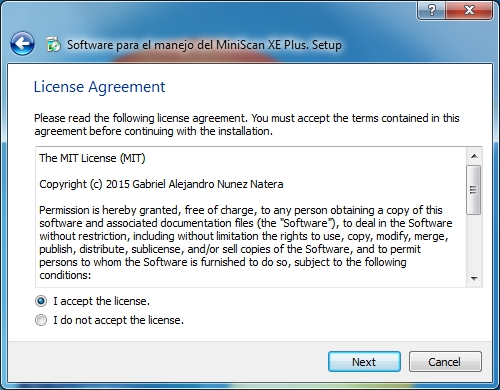
\includegraphics[width=.5\linewidth]{./img/spectrasoft-licencia.jpg}
\caption[Licencia del Spectrasoft]{Licencia del Spectrasoft\label{fig:spectrasoft-licencia}}
\end{figure}

\newpage

En la ventana <<Ready to Install>> haga click en el bot\'{o}n <<Install>> (v\'{e}ase la figura \ref{fig:spectrasoft-instalar}).

\begin{figure}[H]
  \centering
  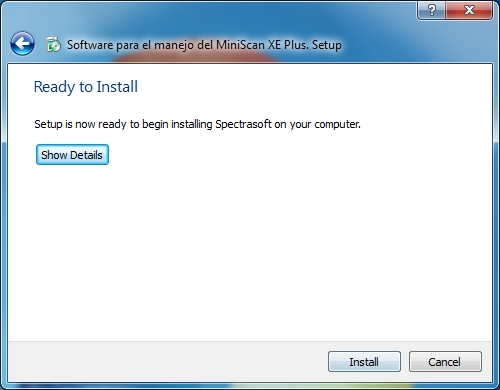
\includegraphics[width=.6\linewidth]{./img/spectrasoft-instalar.jpg}
\caption[Instalar el Spectrasoft]{Instalar el Spectrasoft\label{fig:spectrasoft-instalar}}
\end{figure}

En la ventana <<Completing the Spectrasoft Wizard>> haga click en el bot\'{o}n <<Finish>> (v\'{e}ase la figura \ref{fig:spectrasoft-finalizar}).

\begin{figure}[H]
  \centering
  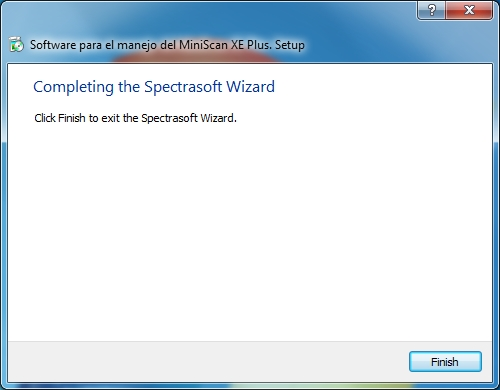
\includegraphics[width=.6\linewidth]{./img/spectrasoft-finalizar.jpg}
\caption[Finalizar la instalaci\'{o}n]{Finalizar la instalaci\'{o}n\label{fig:spectrasoft-finalizar}}
\end{figure}

\newpage

Por \'{u}ltimo, para ejecutar el Spectrasoft abra el men\'{u} de inicio de Windows y haga click en la opci\'{o}n <<Spectrasoft>> (v\'{e}ase la figura \ref{fig:spectrasoft-ejecutable}).

\begin{figure}[H]
  \centering
  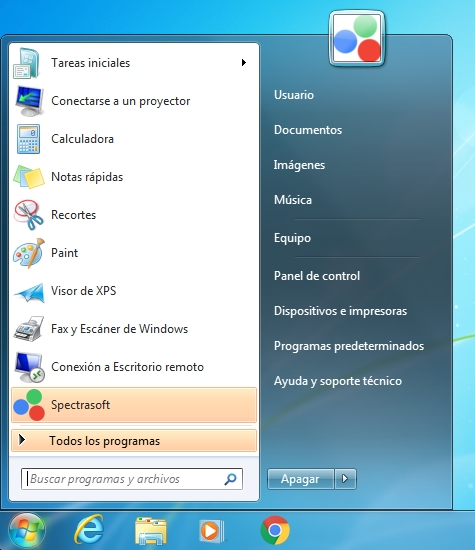
\includegraphics[width=.4\linewidth]{./img/spectrasoft-ejecutable.jpg}
\caption[Ejecutar el Spectrasoft]{Ejecutar el Spectrasoft\label{fig:spectrasoft-ejecutable}}
\end{figure}

Si desea entrar al men\'{u} del Spectrasoft, abra el men\'{u} de inicio de Windows, haga click en la opci\'{o}n <<Todos los programas>>, busque la carpeta llamada <<Spectrasoft>> y seleccionela (v\'{e}ase la figura \ref{fig:spectrasoft-menu}).

\begin{figure}[H]
  \centering
  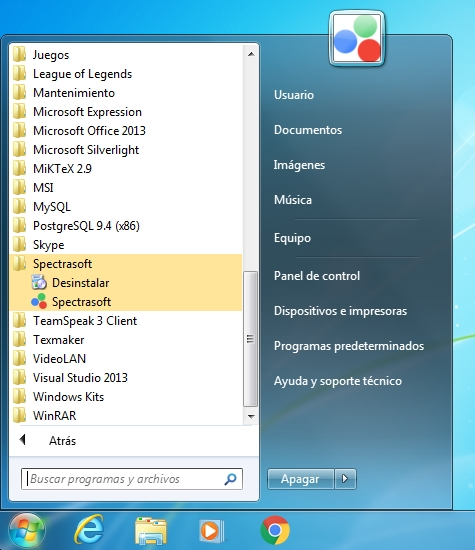
\includegraphics[width=.4\linewidth]{./img/spectrasoft-menu.jpg}
\caption[Men\'{u} del Spectrasoft]{Men\'{u} del Spectrasoft\label{fig:spectrasoft-menu}}
\end{figure}